\documentclass[a4paper,12pt]{article}
\usepackage{cmap}
\usepackage[utf8]{inputenc}
\usepackage[warn]{mathtext}
\usepackage{epsf,amsmath,amsfonts,amssymb,amsbsy}
\usepackage[mathscr]{eucal}
\usepackage[english, russian]{babel}
\usepackage[left=2cm,right=2cm,top=2cm,bottom=2cm]{geometry}
\usepackage{graphicx}
\usepackage{wrapfig}
\usepackage{indentfirst}
\graphicspath{{picture/}}
\DeclareGraphicsExtensions{.pdf,.png,.jpg}
\usepackage{pgfplots}
\usepackage{rotating}
\usepackage{pgfplotstable}
\usepackage{booktabs}
\usepackage{xcolor}
\usepackage{hyperref}
\usepackage{multirow}
\begin{document}

% начало документа
% НАЧАЛО ТИТУЛЬНОГО ЛИСТА
\begin{center}
	\hfill \break
	\hfill \break
	{\small ФЕДЕРАЛЬНОЕ ГОСУДАРСТВЕННОЕ АВТОНОМНОЕ ОБРАЗОВАТЕЛЬНОЕ\\ УЧРЕЖДЕНИЕ ВЫСШЕГО ОБРАЗОВАНИЯ\\ МОСКОВСКИЙ ФИЗИКО-ТЕХНИЧЕСКИЙ ИНСТИТУТ\\ (НАЦИОНАЛЬНЫЙ ИССЛЕДОВАТЕЛЬСКИЙ УНИВЕРСИТЕТ)\\ ФИЗТЕХ-ШКОЛА РАДИОТЕХНИКИ И КОМПЬЮТЕРНЫХ ТЕХНОЛОГИЙ}\\

	\hfill \break
	\normalsize{Лабораторная работа по программированию. }\\
	\vspace{7em}
	\normalsize{\textbf{По теме}}\\
	\vspace{7em}
	\large{<<Ускорение работы хэш-таблицы>>}\\
\end{center}

\vspace{16em}
\begin{flushright}
	\normalsize{Студента 1 курса группы Б01-003}\\
	\normalsize{\textbf{Крейнина Матвея Вадимовича}}\\
\end{flushright}

\vspace{\fill}
\begin{center}
	\normalsize{\textbf{Долгопрудный, 2021}}
\end{center}


\thispagestyle{empty} % выключаем отображение номера для этой страницы
\newpage
% КОНЕЦ ТИТУЛЬНОГО ЛИСТА

	
	\begin{center}
		{\Large Исследование эффективности работы хэш-функций}
	\end{center}
	\section*{Цель работы:}
Оптимизировать хэш таблицы любыми доступными средствами. 

\section*{В работе используются:}
Кривые руки Матвея Крейнина, классы list и line, написанные им же в 1-м семестре, Visual Studio с её прекрасным, красивым и невообразимым профилировщиком, хорошее настроение и любовь к программированию. Все тесты проводились при максимальной производительности ноутбука, подключенного к зарядному устройству и в режиме оптимизации компилятора o2.

\section*{Теоретическое введение:}
Это секретная информация, которую нельзя разглашать.
Возможно, вы сможете найти ответ в книге человека, которого нельзя называть.

\section*{Ход работы:}
1. Для начала я решил измерить время работы своей программы, загрузив в хэш таблицу англо-русский словарь на 158 тысяч слов. Далее я ищу каждое из слов по несколько раз с целью того, чтобы найти <<узкое горлышко>> в своей программе.

\begin{center}
	\begin{figure}[h]
		\caption{Режим компилятора -- o2, время исполнения = 180 мс}
	\end{figure}
	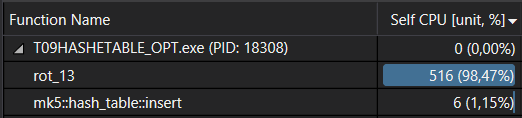
\includegraphics[scale = 1]{1_test.png}
\end{center}

Я нашел узкое место - это вызов функции rot\_13, я перешел в неё и обнаружил, что в цикле я каждый раз считаю длину строки для сравнения.

Я вынес подсчёт длины строки из цикла и получил следующие показатели:

\begin{center}
	\begin{figure}[h]
		\caption{Режим компилятора -- o2, время исполнения = 43 мс}
	\end{figure}
	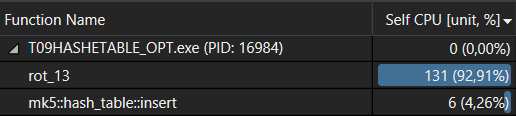
\includegraphics[scale = 1]{2_test.png}
\end{center}
Теперь доля функции rot\_13 снизилась с 98.47\% до 92.91\%, что даже очень хорошо, но можно лучше. При этапе чтения англо-русского словаря, я теперь буду запоминать длину строки и сохраняю её для каждого элемента и теперь её считать не нужно.
\begin{center}
	\begin{figure}[h]
		\caption{Режим компилятора -- o2, время исполнения = 30 мс}
	\end{figure}
	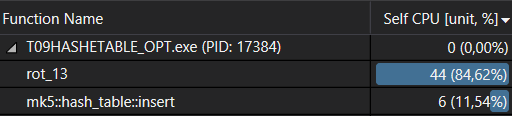
\includegraphics[scale = 1]{3_test.png}
\end{center}

Теперь время работы функции rot\_13 снизилась с 92.91\% до 80.43\% и выросла работа функции insert.

180 мс - время работы с подсчётом строки на каждом шаге,

43 мс - время работы с подсчётом длины строки вне цикла, 

35  мс - время работы с предпосчётом длины строки на этапе загруки.

Благодаря манипуляциям с подсчётом длины строки я получил ускорение в 4.18 раза при подсчёте вне цикла, вероятно, это связано с тем, что строчки у меня короткие, поэтому не так часто их приходится пересчитывать,
в 5.14 раза при подсчёте на этапе загрузки. 
Это уже довольно хороший результат, но нужно двигаться дальше. 

Вооружившись книгой Брайнта-Холларона <<Компьютерные системы архитектура и программирование>>, в пятой по счету главе я нашел, что цикл можно сворачивать выполняя на каждом шаге не одну операцию, а, например, 2. Применив данный метод, для свертывания цикла в два раза я получил - 33 мс, я выиграл 2 мс. Далее я поэксперементировал с 3, 4, 5 и 6, получил соотвественно: 32 мс, 29 мс и 30 мс, 32, больше я не стал продолжать этот опыт, т.к. локальный минимум был найден. 

Погуглив еще немного, я нашел в икстринсиках хэш-функцию - это crc32, я внедрил её в свой проект и получил следующий результат.

\begin{center}
	\begin{figure}[h]
		\caption{Режим компилятора -- o2, время исполнения = 30 мс}
	\end{figure}
	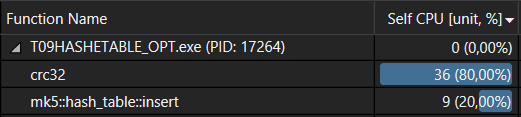
\includegraphics[scale = 1]{4_test.png}
\end{center}


Дальнейшее ускорение программы не представляется возможным, т.к. переписывание хэш функции на икстринсики в первый раз дало проигрыш по времени, а во вторый точно такой же результат, как и оптимизация от Visual Studio, дальнейшее оптимизация функций rot\_13 и crc32 не представляется возможным, по причине того, что подсчёт длины строки оптимизирован и выполняется на этапе загрузки, цикл в подсчёте хэш-функции оптимизирован.

\section*{Вывод}
Я ускорил программу в 6.2 раза в режиме компиляции O2, что является хорошим результатом, т.к. оптимизатор visual studio является одним из лучших.
Теперт нужно подсчитать самое главное число

\section*{Список литературы}
1. Язык программирования СИ, Брайан Керниган и Деннис Ритчи

2. Компьютерные системы архитектура и программирование, Брайнт-Холларон

3. \href{http://ded32.net.ru}{Дединский Илья Рудольфович http://ded32.net.ru}

Возможно, вы заходите заняться компутерной графикой и тогда вы сможете найти одну библиотеку, которая сможет вам помочь.

4. \href{https://www.google.ru}{Google https://www.google.ru }
\end{document}